\chapter{Introduction}
The title of this thesis involves several concepts, plasma, spectral instability, and magnetic nozzle. In the first chapter, we will introduce these concepts. Starting from the definition of plasma, then to the spectral instability and the general procedure of analyzing spectral instability. Following that, magnetic nozzle and magnetic mirror configuration will be introduced. After having these necessary knowledge, we are able to discuss the methods for analyzing the spectral instability of plasma flow in magnetic nozzle.

\section{Plasma}
Plasma is one of the fundamental states of matter, distinct from solid, liquid, and gas. In a plasma, the atoms or molecules have been stripped of electrons, resulting in a collection of charged particles, ions and electrons. In a vigorous sense, plasma is a fourth state of matter, though people often call it that way, because it does not involve phase transition. Plasma is the most common matter in the universe, it can be found in stars, including the sun, where nuclear fusion occurs at extremely high temperature. It also exists in solar wind, lightning and auroras. These natural plasmas can be seen in the sky because they are in plasma state, and plasma is capable of emitting light \cite{chen_introduction_2016}. Plasma has various scientific and technology uses. The artificially generated plasma can be found in fluorescent lights, Neon signs, etc. It can also be found in plasma physics research, nuclear fusion experiments, plasma cutting and welding, plasma medicine for treating diseases, and even in spacecraft propulsion systems. Overall, plasma is an intriguing and versatile state of matter with significant implications in various fields of science, technology, and industry. Fig.~\ref{fig:plasma-properties} lists some commonly seen natural and artificial plasmas.

\begin{figure}[htbp]
	\centering
	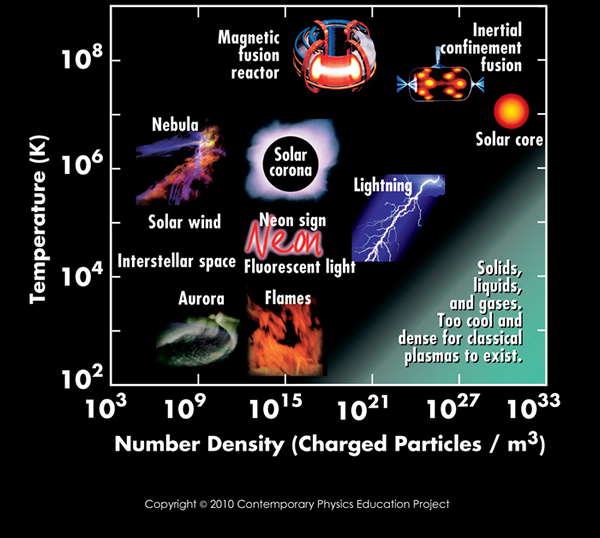
\includegraphics[width=0.7\textwidth]{figures/plasma-properties}
	\caption{Typical plasmas. Adapted from \cite{cpep_physics}.}
	\label{fig:plasma-properties}
\end{figure}

\subsection{Definition of Plasma}
In simple terms, a plasma is an ionized gas which is quasineutral and exhibits collective behavior \cite{chen_introduction_2016}. The following subsections will give precise definition of quasineutrality and collective behavior.

\subsubsection*{Debye Shielding and Quasineutrality}
A key characteristic of plasma is its capability to shield external electric field. Imagine a positively charged ball is put into a plasma (Fig.~\ref{fig:debye-shielding}, ions are neglected from the figure). Suppose there is sufficient amount of electrons in the plasma, and the plasma is cold, meaning that no thermal motions exist, the electric field generated by the ball will be shielded out by the surrounding electron cloud. If the plasma has finite temperature, then due to the thermal motions of electrons, the shielding will be incomplete and the edge of the electron cloud will be at the radius where potential energy is approximately equal to the thermal energy $KT$ \cite{chen_introduction_2016}.

\begin{figure}[htbp]
	\centering
	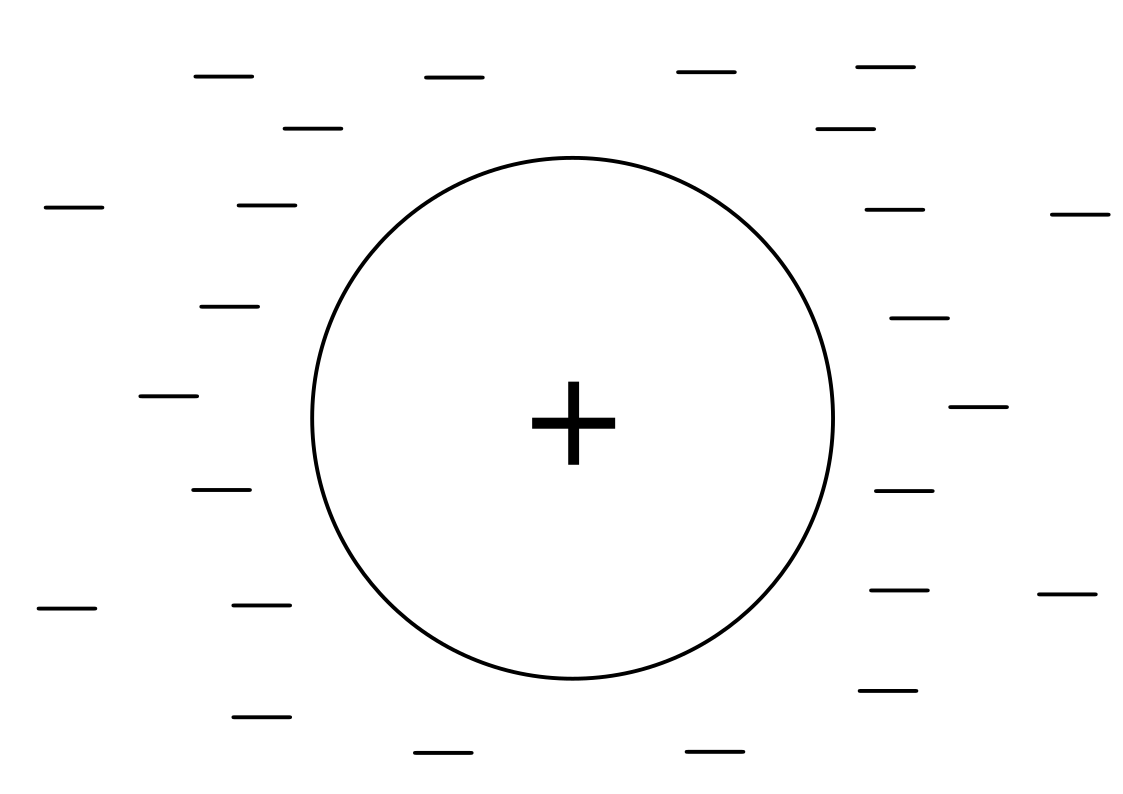
\includegraphics[width=0.4\textwidth]{figures/debye-shielding.png}
	\caption{Debye shielding. Adapted from \cite{chen_introduction_2016}. A positively charged ball is put into a plasma. Electrons will surround the ball. Ions are neglected from the picture since they are repelled away from the ball.}
	\label{fig:debye-shielding}
\end{figure}

The Debye length is the thickness of the electron cloud. To find out Debye length, we need to compute the potential near the positively charged ball. Due to the symmetry of the problem, we can reduce the it to 1D, along the radial direction. Suppose the coordinate's origin is at the ball's center and $\phi(0)=0$. The potential can be solved from the following 1-dimensional Poisson's equation,
\begin{equation}
	\epsilon_0\dv[2]{\phi}{x} = -e(n_i - n_e), \quad \phi(0) = \phi_0.
	\label{eq:poisson-equation-1d}
\end{equation}
Where $n$ is the number density of the particles, and the subscripts $i$ and $e$ stand for ion and electron.

For simplicity, we assume massless electron, $m/M \to 0$. This means that the electrons move so fast that the ions can be treated as a static background. That is,
\begin{equation}
	n_i = n_0.
	\label{eq:ion-density-static-background}
\end{equation}
Where $n_0$ is a constant.

Meanwhile, it can be proven using Fluid description of plasma that the electron density follows the Boltzmann distribution \cite{chen_introduction_2016},
\begin{equation}
	n_e = n_0\exp(e\phi/KT_e).
\end{equation}

Taylor expand $n_e$ in the region where $\abs{e\phi/KT_e} \ll 1$ we have,
\begin{equation}
	n_e = n_0\left[ 1 + \frac{e\phi}{KT_e} + \frac{1}{2}\left(\frac{e\phi}{KT_e}\right)^2 + \cdots \right].
	\label{eq:electron-density-taylor-expansion}
\end{equation}

Substituting Eq.~(\ref{eq:ion-density-static-background}) and Eq.~(\ref{eq:electron-density-taylor-expansion}) for $n_i$ and $n_e$ in the 1D Poisson's equation, Eq.~(\ref{eq:poisson-equation-1d}), and only keep the linear terms in Eq.~(\ref{eq:electron-density-taylor-expansion}), we get
\begin{equation}
	\epsilon_0\dv[2]{\phi}{x} = \frac{n_0e^2}{KT_e}\phi.
\end{equation}

The solution to the Poisson's equation is therefore
\begin{equation}
	\phi = \phi_0\exp(-\abs{x}/\lambda_D).
\end{equation}
Where the quantity $\lambda_D$ is called Debye length, and is defined as
\begin{equation}
	\lambda_D \equiv \left(\frac{\epsilon_0 KT}{ne^2}\right)^{1/2}.
	\label{eq:debye-length}
\end{equation}
Where $n$ stands for the number density far away from the charged ball. The potential is shown in Fig.~\ref{fig:debye-potential}. The  Debye length characterizes the thickness the of the cloud.

\begin{figure}[htbp]
	\centering
	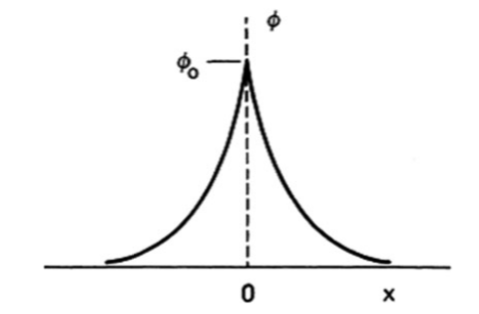
\includegraphics[width=0.7\textwidth]{figures/debye-potential.tikz}
	\caption{Potential distribution near a positively charged ball in a plasma. Adapted from \cite{chen_introduction_2016}. The charged ball is centered at the origin, the potential generated by this ball decreases exponentially.}
	\label{fig:debye-potential}
\end{figure}

The above discussion indicates that any external electric field present in a plasma will be shielded out within a distance $\lambda_D$ (assuming the system size $L$ is much larger than $\lambda_D$). Therefore, the plasma stays neutral if it is initially electrically neutral.

A plasma is said to be quasineutral, if a plasma is neutral enough so that we can take $n_i \simeq n_e$ but a small charge imbalance can give rise to potentials of the order of $KT/e$. In this case, we can the symbol $n$ to denote the common density and call it the plasma density \cite{chen_introduction_2016}.

\subsubsection*{Plasma Oscillation}
Simply speak, the collective behavior of a plasma is mostly governed by the electromagnetic forces rather than the gas dynamics. To quantify this statement, we introduce the concept of plasma oscillation.

There are many kinds of oscillations in plasma, one of the most fundamental oscillations is the electron plasma oscillation. Imagine the ions are too heavy to move, and they form a uniform background. The electrons are then released from a distance away from the ions (Fig.~\ref{fig:plasma-oscillation}). The electric field will pull the electrons toward the ions, after the electrons pass the ions, the electric field will decelerate them and started to pull them on the other side. The frequency of this oscillation is called plasma frequency,
\begin{equation}
	\omega_p = \left(\frac{n_0e^2}{\epsilon_0m}\right)^{1/2}.
\end{equation}

\begin{figure}[htbp]
	\centering
	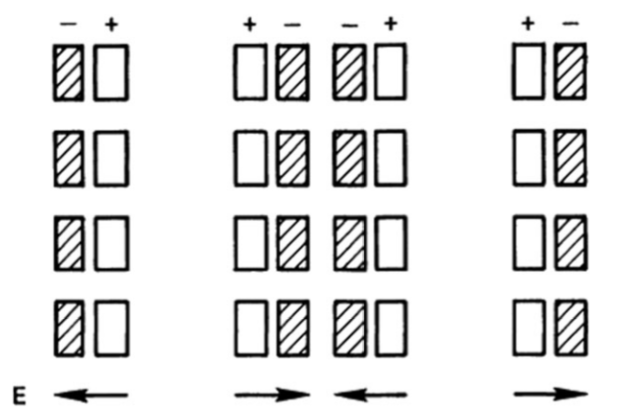
\includegraphics[width=0.7\textwidth]{figures/plasma-oscillation.tikz}
	\caption{Mechanism of plasma oscillations. Adapted from \cite{chen_introduction_2016}. As the electrons are pulled away from the ions, electric field forms and will pull the electrons back to the equilibrium position. Hence oscillation happens.}
	\label{fig:plasma-oscillation}
\end{figure}

\subsubsection*{Criteria of Plasma}
We are now able to give more detail definition for plasma. According to \cite{chen_introduction_2016}, not all ionized gas can be called plasma, there are three conditions a plasma must satisfy:
\begin{enumerate}
	\item Debye length is much smaller than the system size, $\lambda_D \ll L$.
	\item Collective behavior requires lots of particles in a Debye sphere, $N_D = n\frac{4\pi}{3}\lambda_D^3 \ggg 1$.
	\item The ionized gas behaves like plasma rather than a neutral gas, $\omega_p\tau > 1$ where $\omega_p$ typical plasma oscillation frequency and $\tau$ is the mean free time of collisions between neutral atoms.
\end{enumerate}


\section{Instability} \label{sec:instability-of-plasma-flow}
Magnetic nozzle is one of the most actively researched configurations in plasma propulsion systems, which is being developed for space missions due to their potential for high efficiency and thrust. Understanding and controlling instabilities in the plasma flow within these nozzles is essential for optimizing their performance and achieving efficient propulsion. Investigating instabilities in plasma flow within magnetic nozzles also contributes to our broader understanding of fundamental plasma physics phenomena. For instance, in astrophysics, the solar wind is accelerated by a magnetic mirror configuration similar to that of a magnetic nozzle, suggesting that our methodologies can also be applied to such problems.

\subsection{Plasma Instability}
The instability of plasma refers to the tendency of a plasma system to deviate from an equilibrium state under perturbations or fluctuations. It can be understood as the simple mechanical analogy with a ball on crest / in valley. On the left of Fig.~\ref{fig:stability-visualization} shows us a ball in its equilibrium and it is a stable equilibrium. Small perturbations given to the system will not push the ball far away from the equilibrium position, the valley. If friction exists, the ball oscillates with decreasing amplitude and will eventually reached the equilibrium state as time goes to infinity. Hence, the equilibrium is stable. On the right, any small perturbations will cause the ball to fall downhill and will never come back to the initial equilibrium position. Hence this equilibrium is unstable.

\begin{figure}[htbp]
	\centering
	\begin{subfigure}[b]{0.5\textwidth}
		\centering
		\includegraphics[width=0.7\linewidth]{figures/stability-visualization-stable.tikz}
		\caption{Stable equilibrium.}
	\end{subfigure}%
	\begin{subfigure}[b]{0.5\textwidth}
		\centering
		\includegraphics[width=0.7\linewidth]{figures/stability-visualization-unstable.tikz}
		\caption{Unstable equilibrium.}
	\end{subfigure}
	\caption{Mechanical analogy of various types of equilibrium. Adapted from \cite{chen_introduction_2016}.}
	\label{fig:stability-visualization}
\end{figure}


The instabilities in plasma can arise from various factors, such as the interaction of particles with electromagnetic fields, collective effects, or the presence of gradients in plasma parameters. A famous example of instability is the two stream instability. The configuration starts with two oppositely traveling beams of ions and electrons. As time evolves, the two beams can no longer stay in its equilibrium state due to the electromagnetic interactions, and chaotic behavior develops as shown in Fig.~\ref{fig:two-stream-instability}.

\begin{figure}[htbp]
	\centering
	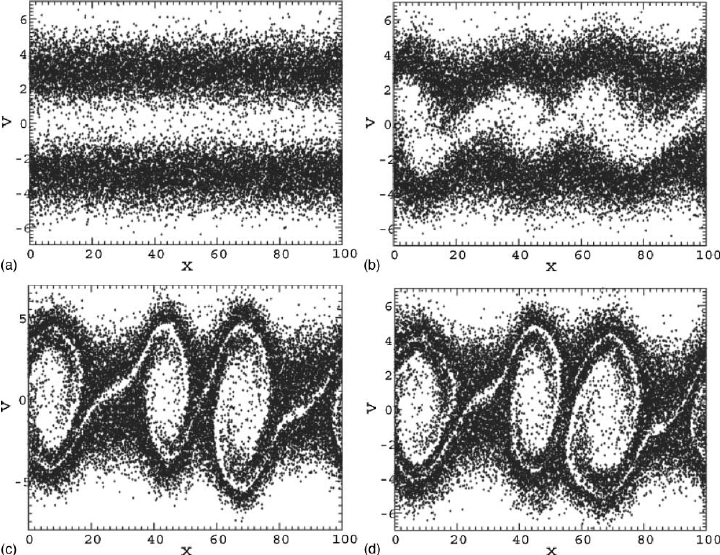
\includegraphics[width=0.7\linewidth]{figures/two-stream-instability}
	\caption{Visualization of two-stream instability in the phase space. (a) Initially the ion and electron flow are in opposite direction. (b) The velocity of both flows start to oscillate. (c) Chaotic behavior occurs. (d) The chaotic behavior continues. Adapted from \cite{ha_nonlinear_2011}.}
	\label{fig:two-stream-instability}
\end{figure}

\subsection{Spectral Instability of Partial Differential Equations}
In the study of partial differential equations (PDEs), there are two types of instability: structural instability and dynamic instability. The structural instability refers to the tendency of the solution to diverge under perturbations in the PDE parameters, while the dynamic instability refers to the tendency of solution to deviate from a stationary solution given perturbations in the stationary solution \cite{beck_spectral_2020}. We are interested in the dynamic instability. In this subsection, we will describe the process for investigating plasma instability, and explain why we can investigate the dynamic instability by analyzing the spectrum of the linear operator of the corresponding linearized PDE. Hence the name spectral instability. We will discuss the connection between spectral instability and the plasma instability later in this subsection.

In order to investigate the plasma instability, the first step is to state the governing equations for the plasma flow in the magnetic nozzle. The governing equations are time-dependent fluid equations involving the number density $n$ and fluid velocity $v$ of the plasma flow along the central axis of the nozzle,
\begin{equation}
	\pdv{t}\mqty[n\\ v] + \mathbf{F}(n,v) = \mathbf{0}.
	\label{eq:pde-system}
\end{equation}
This PDE system has two first-order PDEs, Eq.~(\ref{eq:conservation-of-density}) and Eq.~(\ref{eq:conservation-of-momentum}). Detail derivation will be given in Sec.~\ref{sec:equation-of-motion-of-the-plasma-flow-in-nozzle}.

Following this we find the equilibrium state (stationary solution) to the above PDE system, Eq.~(\ref{eq:pde-system}). In other words, we find $n_0$ and $v_0$ such that $\mathbf{F}(n_0,v_0)=\mathbf{0}$. The expression of equilibrium velocity $v_0$ is given by Eq.~(\ref{eq:velocity-profile}) and it can be found in Sec.~\ref{sec:velocity-profiles}. The details of derivation and Lambert-W will be explained in Sec.~\ref{sec:velocity-profiles}. As for $n_0$, it is not required to obtain its expression because we are able to reduce the linearized first-order PDE system Eq.~(\ref{eq:pde-system}) into a second-order PDE by eliminating the density $n$.

Now we are in a stage ready to investigate the dynamic instability of the problem. The system will be given small spatial perturbations, they serve as small fluctuations on number density and velocity, $\tilde{n}(z)$ and $\tilde{v}(z)$. All variables $n$ and $v$ in the governing equations will be substituted by perturbed quantities, $n_0+\tilde{n}$ and $v_0+\tilde{v}$. The PDE system Eq.~(\ref{eq:pde-system}) now becomes,
\begin{equation}
	\underbrace{\pdv{t}\mqty[\tilde{n}\\ \tilde{v}] + d\mathbf{F}(n_0,v_0)\mqty[\tilde{n}\\ \tilde{v}] }_{\text{linear terms}}
	+ \underbrace{\mathbf{F}(n_0+\tilde{n}, v_0+\tilde{v}) - d\mathbf{F}(n_0,v_0)\mqty[\tilde{n}\\ \tilde{v}]}_{\text{non-linear terms}}
	= \mathbf{0}.
	\label{eq:perturbed-pde-system}
\end{equation}
Where $d\mathbf{F}$ is a Jacobian matrix. Since $\tilde{n}$ and $\tilde{v}$ are small, we expect the higher order mixed terms such as $\tilde{n}\tilde{v}$, $\tilde{n}\partial_z\tilde{v}$, $\tilde{v}\partial_z\tilde{n}$ are negligible comparing to the linear terms. So we drop the non-linear terms. Now we obtain the so-called linearized governing equations, they are the linearized conservation of density, Eq.~(\ref{eq:linearized-conservation-of-density}) and the linearized conservation of momentum, Eq.~(\ref{eq:linearized-conservation-of-momentum}), respectively.

Since we are dealing with linear operators, let the perturbations take the form of exponential $\exp(-i\omega t)$. This indicates that physically the perturbations are oscillating with frequency $\omega$ in time. Any time derivative on the perturbations in the linearized governing equations simply becomes $\partial_t \to -i\omega$. Now we obtain equations involving perturbations, $\tilde{n}$ and $\tilde{v}$, and their spatial derivatives, and $\omega$. Reducing the number of equations by eliminating the density $\tilde{n}$, we obtain Eq.~(\ref{eq:polynomial-eigenvalue-problem}).

The problem of investigating the plasma instability becomes the problem of finding the eigenvalues, $\omega$, of Eq.~(\ref{eq:polynomial-eigenvalue-problem}) under different boundary conditions. The connection between the eigenvalue $\omega$ and the plasma instability is clear: The oscillation frequency $\omega$ is a complex number. If the imaginary part of the temporal frequency is greater than zero, i.e. $\Im(\omega) > 0$, then the system is unstable. This is because the perturbation grows exponentially $\exp(\Im(\omega)t)$ in time. On the other hand, if the imaginary part of the temporal frequency is less than or equal to zero, $\Im(\omega) \leq 0$, then the system is said to be stable. Since the perturbations will not be growing, $\Im(\omega)=0$, or even damped, $\Im(\omega) < 0$.

Since the PDE we analyze is linear, its spectral instability is also called linear instability. In this following thesis, the terms plasma instability, spectral instability, linear instability will be used interchangeably, sometimes an even shorter term instability will be used.

We will devote the rest of the chapters to develop methods for solving the eigenvalue problem Eq.~(\ref{eq:polynomial-eigenvalue-problem}). We will employ spectral methods to obtain eigenvalues for subsonic and supersonic velocity profiles, and shooting method will be used to get eigenvalues when velocity profile $v_0$ is accelerating.

\section{Magnetic Nozzle}
In this thesis, we are going to deal with plasma flow in magnetic nozzle.
A magnetic nozzle is a device that uses a magnetic field to shape and control the flow of charged particles in a plasma propulsion system, see Fig.~\ref{fig:magnetic-nozzle}. By employing magnetic mirrors, the magnetic nozzle can efficiently direct and accelerate the plasma particles, generating thrust for propulsion. The magnetic field in the nozzle helps collimate and focus the plasma exhaust, increasing its velocity and enhancing the performance of the propulsion system.

\begin{figure}[htbp]
	\centering
	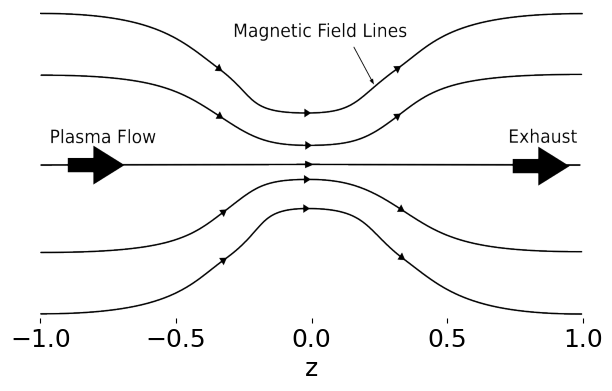
\includegraphics[width=0.7\linewidth]{figures/magnetic-nozzle.png}
	\caption{A simplified example of a magnetic nozzle configuration. On the left ($z=-1$) is the entrance of the nozzle. The plasma flows into the nozzle from the left and will be accelerated and finally exhaust through the exit on the right ($z=1$). The magnetic field lines are shaped in such a way that it forms a magnetic mirror configuration. Plasma flow with specific subsonic speed at the entrance will be accelerated to supersonic speed.}
	\label{fig:magnetic-nozzle}
\end{figure}

\subsection{Magnetic Field in Magnetic Nozzle} \label{sec:magnetic-field-in-nozzle}
The magnetic nozzle by its nature is 3-dimensional. We assume the magnetic field is axis-symmetric, then the radial magnetic field and axial magnetic field are constraint by divergence-free condition,
\begin{equation}
	\div\mathbf{B} = \frac{1}{r}\pdv{(rB_r)}{r} + \pdv{B_z}{z} = 0.
	\label{eq:divergence-free-condition}
\end{equation}

Since we are interested in the plasma flow near the central axis of the nozzle, with paraxial approximation taken, the derivative along the magnetic field line $\nabla_\parallel = \pdv*{z}$ when near the central axis \cite{smolyakov_quasineutral_2021}. Hence, in this thesis we will treat the flow in magnetic nozzle as a 1-dimensional problem. The axial magnetic field along the central axis is modeled as
\begin{equation}
	B_z(z) = B_0 \left[1 + R\exp(-\left(\frac{z}{\delta}\right)^2)\right], \quad -1\leq z \leq 1.
\end{equation}
Where $1+R$ is the magnetic mirror ratio, it is the ratio of the magnitude of magnetic field at the center of the nozzle to that at the end of the nozzle, $1+R = B(0)/B(1)$. The mirror ratio $R$ controls the spread of the plasma flow at the exit. On the other hand, $\delta$ determines the spread of the magnetic field. Larger the $\delta$, flatter the magnetic field. An example of magnetic field is shown in Fig.~(\ref{fig:magnetic-field}).

The radial profile of magnetic field, $B_r$, is given by the divergence-free condition, Eq.~(\ref{eq:divergence-free-condition}). In this thesis will focus on the axial magnetic field only.

\begin{figure}[htbp]
	\centering
	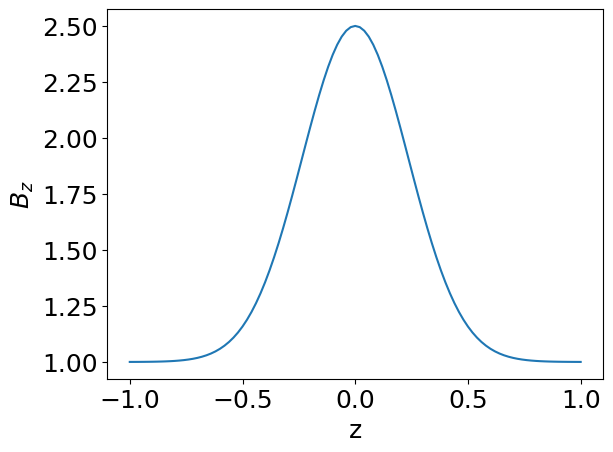
\includegraphics[width=0.7\linewidth]{figures/magnetic-field}
	\caption{This is the magnetic field in nozzle with mirror ratio $1+R=B_{max}/B_{min}=2.5$, and the spread of magnetic field, $\delta=0.1/0.3=0.\bar{3}$. }
	\label{fig:magnetic-field}
\end{figure}

\subsection{Velocity Profiles of Plasma Flow in Magnetic Nozzle}
The analytical solution gives 4 different kinds of velocity profiles,
\begin{itemize}
	\item Subsonic profile: Plasma flow enters and exits the nozzle with subsonic speed. Every point on this profile is subsonic.
	\item Supersonic profile: Plasma flow enters and exits the nozzle with supersonic speed. Every point on this profile is supersonic.
	\item Accelerating profile: Plasma flow enters the nozzle with subsonic speed and exits the nozzle with supersonic speed. Points before the nozzle throat are subsonic, and the flow reaches ion sound speed at the nozzle throat, then the flow is supersonic after the nozzle throat.
	\item Decelerating profile: Plasma flow enters the nozzle with supersonic speed and exits the nozzle with subsonic speed. Similar to the accelerating profile, but the velocity is decreasing.
\end{itemize}
See Fig.~\ref{fig:velocity-profiles} for these profiles.

The velocity of plasma flow in the magnetic nozzle is given by the Lambert W function, Eq.~(\ref{eq:velocity-profile}). The Lambert W function has 2 different branches. The $k=0$ branch corresponds to the subsonic parts in the velocity profile, and the $k=-1$ branch gives the supersonic parts. The expression of velocity profile will be derived in Chap.~\ref{chap:fluid-equations} and more details will be discussed.

\section{Flow in Similar Configuration: Bondi-Parker Flow}
Consider a massive celestial object in the space. This celestial object will attract matter in the space because it is massive. Hence, creating an accretion flow. If the celestial object is a star, it can also eject matter into space. Solar wind is an example to this since it is a stream of charged particles, primarily electrons and protons, flowing outward from the Sun. Bondi derived a steady-state solution for accretion flow which is governed by Bernoulli's equation in spherical symmetry around a point mass in 1952. Hence, the inward accretion flow is also called Bondi flow. Then Parker solved a similar problem but with outward wind in 1958. Then the outward wind is given the name, Parker flow \cite{aikawa_stability_1979,bondi_spherically_1952,keto_stability_2020}. The Bondi and Parker flow (also called Bondi-Parker flow) is similar to that in magnetic nozzle. It is interesting to compare the two configurations.

If we compare the velocity profiles for Bondi-Parker flow and the flow in magnetic nozzle. We found they are similar. The Bondi-Parker flow can also be grouped into the following types: subsonic, supersonic, and transonic (accelerating and decelerating). See Fig.~\ref{fig:BP-flow-velocity}. For subsonic profiles, every point on the curve is slower than sound speed. While every point on the supersonic velocity profile is faster than sound speed. Lastly, there are two different transonic profiles: accelerating profile and decelerating profile. The accelerating profile describes the accelerating plasma flow which is at subsonic speed at the mass point, e.g. a star, and is accelerated to supersonic speed far away. The decelerating profile shows that a plasma flow ejected supersonically from a mass point and then decelerated to subsonic speed far away.

The velocity profiles of one-dimensional, spherically symmetric, stationary isothermal Parker flow neglecting self-gravity can be expressed using Lambert W function,
\begin{equation}
	v(r) = \sqrt{-\frac{KT}{m}W_k\left[ -\left(\frac{r}{r_c}\right)^2 \exp\left[4\left(1-\frac{r_c}{r}\right)-1\right] \right]}, \quad
	k = 0,-1.
\end{equation}
Where $r$ stands for the distance measured from the center of the mass point, e.g. star. The position $r_c=GMm/2KT$ is the critical position and the velocity at this point is exactly the sonic speed $v(r_c)=\sqrt{KT/m}$, where $M$ is the mass of the mass point, $m$ is the mass of a single particle in the flow, and $T$ is the temperature of the flow. The Bondi flow is simply $-v(r)$ since it is accretion flow, the particles are flowing inwardly towards the mass point.

As we can see the expression of velocity profile for Bondi-Parker flow is similar to that of the magnetic nozzle, Eq.~(\ref{eq:velocity-profile}). The expression is governed by the Lambert W function. Similarly, the $k=0$ branch corresponds to the subsonic part in the velocity profile, and the $k=-1$ branch corresponds to the supersonic part of the profile.

\begin{figure}[htbp]
	\centering
	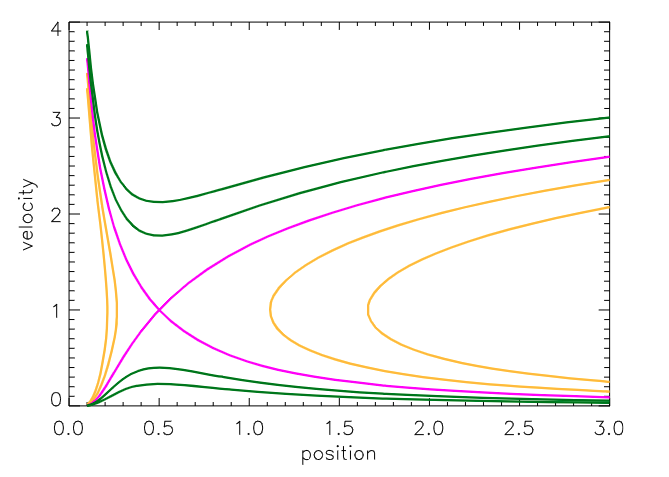
\includegraphics[width=0.7\textwidth]{figures/steady-state-BP-flow}
	\caption{Representative trajectories of the steady-state BP flow in non-dimensional units. The velocities are shown in absolute values. Adapted from \cite{keto_stability_2020}. The upward pink line represents an accelerating flow, it accelerates from subsonic to supersonic. The downward pink line represents a decelerating flow. The green lines below the pink lines represent subsonic flows, and the green lines above represent supersonic flows. Orange lines are physically impossible scenarios. If the sign of the velocity is positive, then it is an outward (Parker) flow, otherwise it is an inward (Bondi) flow.}
	\label{fig:BP-flow-velocity}
\end{figure}

The instabilities of the Bondi-Parker flow has been extensively studied \cite{bondi_spherically_1952,velli_from_1994,velli_hydrodynamics_2001,del_dynamical_1998,keto_stability_2020}. Hopefully these studies can provide insights into our problem.

\section{Goals of this Thesis}
Fusion is considered the next-generation source of a clean, safe and abundant energy providing an opportunity to address climate change problems. A new high-tech industry has appeared in the last decade fueled by over \$4 billion of private investments, with the second world largest and several other smaller companies founded in Canada. To achieve controlled fusion, one of the key science problems is to understand and learn to predict the non-linear behavior of plasma due to waves and instabilities. The general objective of my research is to understand the behavior and learn to control the turbulent flows of plasmas in magnetically controlled fusion system, in particular, open magnetic mirrors. I study the instabilities of the flow in a magnetic mirror configuration under different boundary conditions which is an open question and is under debate in application to fusion systems and also related to the solar wind flows.

The general objective of this research is to understand the instability of the flow in a magnetic nozzle. Plasma confined by the magnetic field is typically far from the state of the thermodynamic equilibrium which makes it unstable. In this project, we would like to investigate the stability of plasma flow in a magnetic nozzle under different boundary conditions. Understanding the instabilities of plasma flow in a magnetic mirror configuration is important in applications such as the expanding magnetic divertors in controlled fusion and electric propulsion \cite{ryutov_divertor_2016,kaganovich_2020_physics}.

In the following thesis, particle and fluid description of plasma will be reviewed in Chap.~\ref{chap:fluid-equations} and linearized governing equations will be derived in the subsequent chapter, Chap.~\ref{chap:polynomial-eigenvalue-problem}. The problem will be then formulated as an eigenvalue problem. In Chap.~\ref{chap:spectral-method}, spectral methods for solving eigenvalue problem will be introduced. Spectral-collocation and spectral-Galerkin methods will be discussed. Moreover, spectral pollution and the filtering techniques will as also be investigated. If the plasma flow in the magnetic nozzle is transonic, the existence of singularity at the nozzle throat prevents the use the spectral methods, therefore we will formulate the problem to the form suitable for applying shooting method. In Chap.~\ref{chap:singular-perturbation} we will discuss the existence of the singularity and then extract the regular solutions using Frobenius method. After this, we will apply shooting method to the problem and investigate the instabilities. Summary of the results and limitations of the methods are discussed in Chap.~\ref{chap:discussion}.

